%!TeX root=../tese.tex
%("dica" para o editor de texto: este arquivo é parte de um documento maior)
% para saber mais: https://tex.stackexchange.com/q/78101/183146

%% ------------------------------------------------------------------------- %%
\chapter{Uma introdução à Teoria dos Grafos}
\label{cap:introducao}

\section{As Pontes de Königsberg}

No século XVIII, a cidade de Königsberg, na Prússia (hoje Kaliningrado, na  atual 
Rússia) era um importante centro comercial devido à sua localização próxima ao rio,
que dividia a cidade em quatro regiões, interligadas por sete pontes.

\begin{figure}
  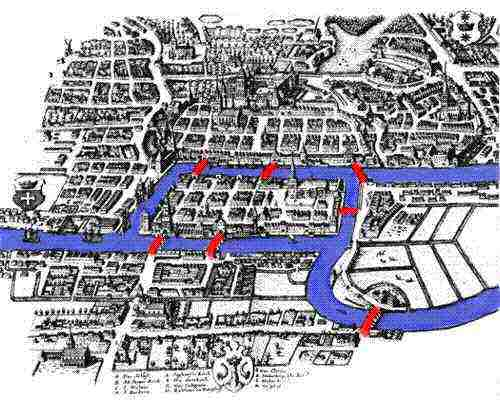
\includegraphics[scale=0.5]{Konigsberg.jpeg}
  \caption{A cidade de Königsberg e suas sete pontes}
\end{figure}

Segundo histórias, um passatempo de domingo dos cidadãos de Königsberg consistia em
passear por sua cidade, até que um dia surgiu um desafio: encontrar uma forma
de andar por todas as regiões passando por cada ponte apenas uma vez.

Nenhum habitante de Königsberg conseguiu encontrar a solução para este problema,
porém, o desafio chegou até um homem chamado Leonhard Euler, que apesar de julgar
o problema trivial, ficou intrigado, como citado em \citet{hopkins04:the}:

\begin{quotation}
  \emph{``This question is so banal, but seemed to me worthy of attention in that 
  [neither] geometry, nor algebra, nor even the art of counting was sufficient to
  solve it.''}
\end{quotation}

Euler provou que não era possível passar por toda a cidade de Königsberg sem passar
duas vezes pela mesma ponte, mas também resolveu o caso geral,
para qualquer número de regiões e qualquer número de pontes, dando assim origem
a um ramo da matemática que hoje chamamos de \textbf{Teoria dos Grafos}.

\section{Grafos}

Podemos definir um \textbf{Grafo} informalmente como um conjunto de entidades
conectadas entre si (ou não). Mais formalmente, podemos definir um grafo $G$ como um
par $(V, E)$ onde $V$ é um conjunto de \textbf{vértices} e $E$ um conjunto de
\textbf{arestas} entre os vértices tal que $E \subseteq \{ (u, v) \mid u, v \in V \}$.

As arestas de um grafo podem ter propriedades como direção e/ou algum valor
associado dependendo do contexto em que está sendo utilizado, frequentemente
possibilitando soluções elegantes e eficientes para os mais diversos problemas.

\begin{figure}
  \centering

  \begin{subfigure}{0.4\textwidth}
    \centering
    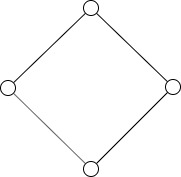
\includegraphics[width=.7\textwidth]{graph.jpg}
    \caption{Um grafo não dirigido.\label{fig:subfigures:a}}
  \end{subfigure}
  % ATENÇÃO: Se você deixar uma linha em branco entre as subfiguras,
  % LaTeX vai considerar que cada uma delas pertence a um "parágrafo"
  % diferente e, portanto, vai colocá-las em linhas separadas ao invés
  % de lado a lado.
  \begin{subfigure}{0.4\textwidth}
    \centering
    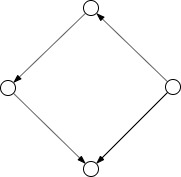
\includegraphics[width=.7\textwidth]{directed_graph.jpg}
    \caption{Um grafo dirigido.\label{fig:subfigures:b}}
  \end{subfigure}

  \begin{subfigure}{0.4\textwidth}
    \centering
    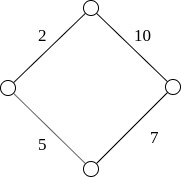
\includegraphics[width=.7\textwidth]{weighted_graph.jpg}
    \caption{Um grafo com valores nas arestas.\label{fig:subfigures:c}}
  \end{subfigure}
  \begin{subfigure}{0.4\textwidth}
    \centering
    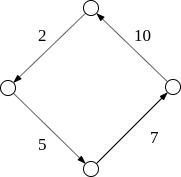
\includegraphics[width=.7\textwidth]{weighted_directed_graph.jpg}
    \caption{Um grafo dirigido com valores nas arestas.\label{fig:subfigures:d}}
  \end{subfigure}

  \caption{Exemplos de grafos.\label{fig:subfigures}}
\end{figure}

\section{Árvores}

\textbf{Árvores} são um subconjunto dos grafos de incrível importância para a
Ciência da Computação, sendo usadas nas mais diversas aplicações, desde a estrutura
de pastas de um sistema operacional até bancos de dados e processamento de
linguagem natural.

Diferente de outras estruturas como vetores, as árvores se organizam de forma
não linear, hierárquica. Os elementos de uma árvore são chamados de \textbf{nós} e
comumente um nó específico é elegido para ser a sua \textbf{raíz}. Cada nó pode
ter ligações com outros nós denominados \textbf{filhos}, que por sua vez podem
ter seus próprios filhos e assim sucessivamente até chegarmos em nós que não
possuem ligação com nenhum outro elemento; chamamos estes nós de \textbf{folhas}.

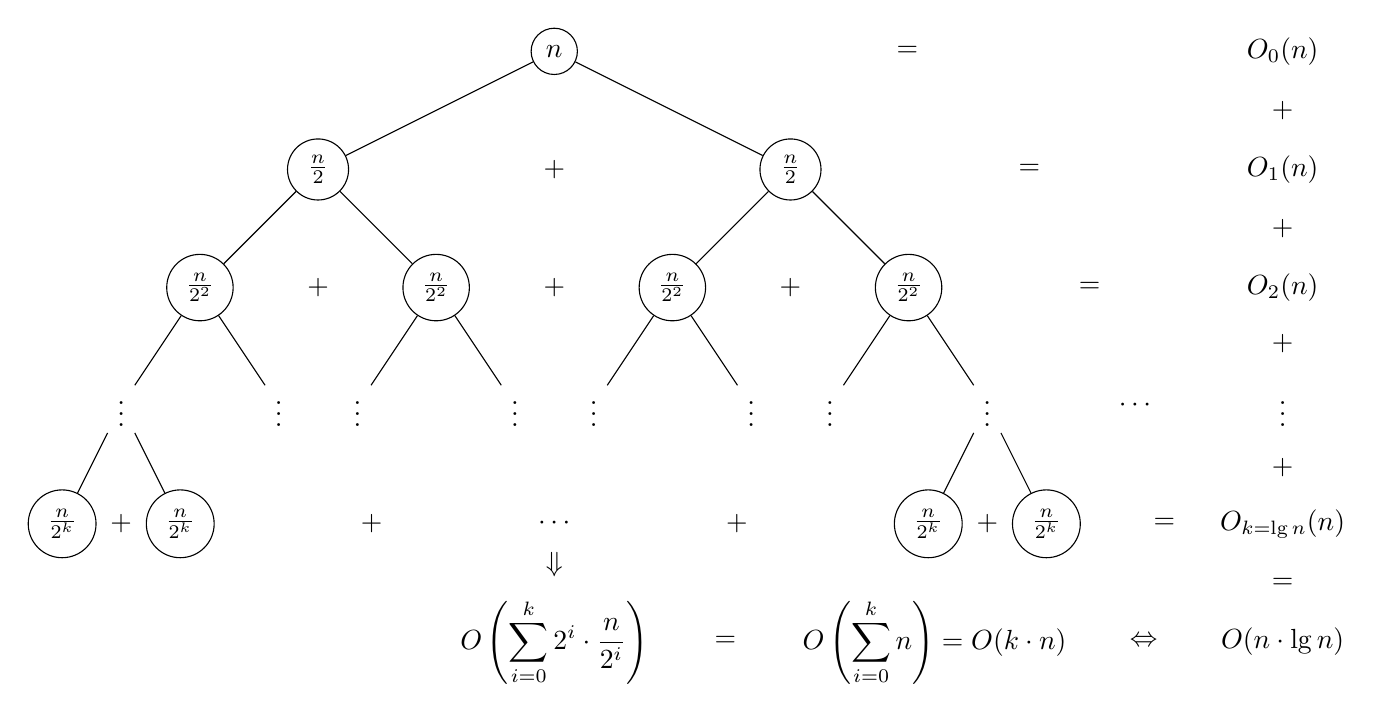
\begin{tikzpicture}[level/.style={sibling distance=60mm/#1}]
\node [circle,draw] (z){$n$}
  child {node [circle,draw] (a) {$\frac{n}{2}$}
    child {node [circle,draw] (b) {$\frac{n}{2^2}$}
      child {node {$\vdots$}
        child {node [circle,draw] (d) {$\frac{n}{2^k}$}}
        child {node [circle,draw] (e) {$\frac{n}{2^k}$}}
      } 
      child {node {$\vdots$}}
    }
    child {node [circle,draw] (g) {$\frac{n}{2^2}$}
      child {node {$\vdots$}}
      child {node {$\vdots$}}
    }
  }
  child {node [circle,draw] (j) {$\frac{n}{2}$}
    child {node [circle,draw] (k) {$\frac{n}{2^2}$}
      child {node {$\vdots$}}
      child {node {$\vdots$}}
    }
  child {node [circle,draw] (l) {$\frac{n}{2^2}$}
    child {node {$\vdots$}}
    child {node (c){$\vdots$}
      child {node [circle,draw] (o) {$\frac{n}{2^k}$}}
      child {node [circle,draw] (p) {$\frac{n}{2^k}$}
        child [grow=right] {node (q) {$=$} edge from parent[draw=none]
          child [grow=right] {node (q) {$O_{k = \lg n}(n)$} edge from parent[draw=none]
            child [grow=up] {node (r) {$\vdots$} edge from parent[draw=none]
              child [grow=up] {node (s) {$O_2(n)$} edge from parent[draw=none]
                child [grow=up] {node (t) {$O_1(n)$} edge from parent[draw=none]
                  child [grow=up] {node (u) {$O_0(n)$} edge from parent[draw=none]}
                }
              }
            }
            child [grow=down] {node (v) {$O(n \cdot \lg n)$}edge from parent[draw=none]}
          }
        }
      }
    }
  }
};
\path (a) -- (j) node [midway] {+};
\path (b) -- (g) node [midway] {+};
\path (k) -- (l) node [midway] {+};
\path (k) -- (g) node [midway] {+};
\path (d) -- (e) node [midway] {+};
\path (o) -- (p) node [midway] {+};
\path (o) -- (e) node (x) [midway] {$\cdots$}
  child [grow=down] {
    node (y) {$O\left(\displaystyle\sum_{i = 0}^k 2^i \cdot \frac{n}{2^i}\right)$}
    edge from parent[draw=none]
  };
\path (q) -- (r) node [midway] {+};
\path (s) -- (r) node [midway] {+};
\path (s) -- (t) node [midway] {+};
\path (s) -- (l) node [midway] {=};
\path (t) -- (u) node [midway] {+};
\path (z) -- (u) node [midway] {=};
\path (j) -- (t) node [midway] {=};
\path (y) -- (x) node [midway] {$\Downarrow$};
\path (v) -- (y)
  node (w) [midway] {$O\left(\displaystyle\sum_{i = 0}^k n\right) = O(k \cdot n)$};
\path (q) -- (v) node [midway] {=};
\path (e) -- (x) node [midway] {+};
\path (o) -- (x) node [midway] {+};
\path (y) -- (w) node [midway] {$=$};
\path (v) -- (w) node [midway] {$\Leftrightarrow$};
\path (r) -- (c) node [midway] {$\cdots$};
\end{tikzpicture}

Também definimos a \textbf{profundidade} de um nó como a quantidade
de arestas no caminho da raíz até ele. A raíz tem profundidade zero,
seus filhos profundidade um e assim sucessivamente.

\begin{figure}
  \centering
  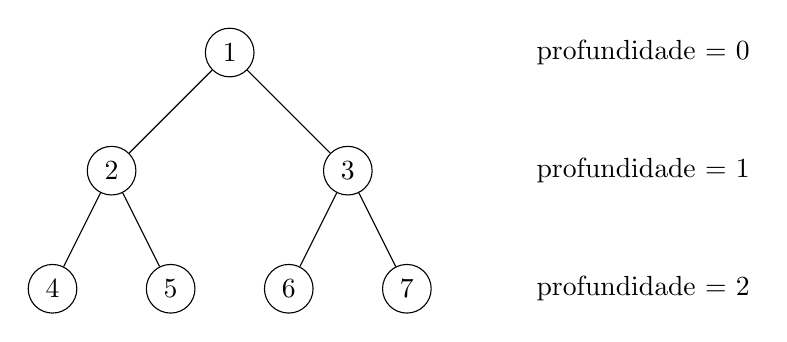
\begin{tikzpicture}[
    level distance=1.5cm,
    level 1/.style={sibling distance=3cm},
    level 2/.style={sibling distance=1.5cm}]
    \node [circle, draw] {1}
      child {node [circle, draw] {2}
        child {node [circle, draw] {4}}
        child {node [circle, draw] {5}}
      }
      child {node [circle, draw] {3}
      child {node [circle, draw] {6}}
        child {node [circle, draw] {7}
        child [grow=right] {node (q) {$\qquad$} edge from parent[draw=none]
            child [grow=right] {node (q) {profundidade = 2} edge from parent[draw=none]
              child [grow=up] {node (r) {profundidade = 1} edge from parent[draw=none]
                child [grow=up] {node (s) {profundidade = 0} edge from parent[draw=none]
                }
              }
            }
          }
        }
      };
  \end{tikzpicture}
  \caption{O nó 1 é a raíz e tem como filhos os nós 2 e 3, cujos
  filhos são as folhas 4, 5 e 6, 7, respectivamente.}
  \end{figure}

\newpage

% Escrever bem é uma arte que exige muita técnica e dedicação e,
% consequentemente, há vários bons livros sobre como escrever uma boa
% dissertação ou tese. Um dos trabalhos pioneiros e mais conhecidos nesse
% sentido é o livro de
% %Umberto Eco~\cite{eco:09} % usando o estilo alpha
% Umberto~\citet{eco:09} % usando o estilo plainnat
% intitulado \emph{Como se faz uma tese}; é uma leitura bem interessante mas,
% como foi escrito em 1977 e é voltado para trabalhos de graduação na Itália,
% não se aplica tanto a nós.

% Sobre a escrita acadêmica em geral, John Carlis disponibilizou um texto curto
% e interessante~\citep{carlis:09} em que advoga a preparação de um único
% rascunho da tese antes da versão final. Mais importante que isso, no
% entanto, são os vários \textit{insights} dele sobre a escrita acadêmica.
% Dois outros bons livros sobre o tema são \emph{The Craft of Research}~\citep{craftresearch}
% e \emph{The Dissertation Journey}~\citep{dissertjourney}. Além disso, a USP
% tem uma compilação de normas relativas à produção de documentos
% acadêmicos~\citep{usp:guidelines} que pode ser utilizada como referência.

% Para a escrita de textos especificamente sobre Ciência da Computação, o
% livro de Justin Zobel, \emph{Writing for Computer Science}~\citep{zobel:04}
% é uma leitura obrigatória. O livro \emph{Metodologia de Pesquisa para
% Ciência da Computação} de
% %Raul Sidnei Wazlawick~\cite{waz:09} % usando o estilo alpha
% Raul Sidnei~\citet{waz:09} % usando o estilo plainnat
% também merece uma boa lida. Já para a área de Matemática, dois livros
% recomendados são o de Nicholas Higham, \emph{Handbook of Writing for
% Mathematical Sciences}~\citep{Higham:98} e o do criador do \TeX{}, Donald
% Knuth, juntamente com Tracy Larrabee e Paul Roberts, \emph{Mathematical
% Writing}~\citep{Knuth:96}.

% Apresentar os resultados de forma simples, clara e completa é uma tarefa que
% requer inspiração. Nesse sentido, o livro de
% %Edward Tufte~\cite{tufte01:visualDisplay}, % usando o estilo alpha
% Edward~\citet{tufte01:visualDisplay}, % usando o estilo plainnat
% \emph{The Visual Display of Quantitative Information}, serve de ajuda na
% criação de figuras que permitam entender e interpretar dados/resultados de forma
% eficiente.

% Além desse material, também vale muito a pena a leitura do trabalho de
% %Uri Alon \cite{alon09:how}, % usando o estilo alpha
% Uri \citet{alon09:how}, % usando o estilo plainnat
% no qual apresenta-se uma reflexão sobre a utilização da Lei de Pareto para
% tentar definir/escolher problemas para as diferentes fases da vida acadêmica.
% A direção dos novos passos para a continuidade da vida acadêmica deveria ser
% discutida com seu orientador.

% %% ------------------------------------------------------------------------- %%
% \section{Considerações de Estilo}
% \label{sec:consideracoes_preliminares}

% Normalmente, as citações não devem fazer parte da estrutura sintática da
% frase\footnote{E não se deve abusar das notas de rodapé.\index{Notas de rodapé}}.
% No entanto, usando referências em algum estilo autor-data (como o estilo
% plainnat do \LaTeX{}), é comum que o nome do autor faça parte da frase. Nesses
% casos, pode valer a pena mudar o formato da citação para não repetir o nome do
% autor; no \LaTeX{}, isso pode ser feito usando os comandos
% \textsf{\textbackslash{}citet}, \textsf{\textbackslash{}citep},
% \textsf{\textbackslash{}citeyear} etc. documentados no pacote
% natbib \citep{natbib}\index{natbib} (esses comandos são compatíveis com biblatex
% usando a opção \textsf{natbib=true}, ativada por padrão neste modelo). Em geral,
% portanto, as citações devem seguir estes exemplos:

% \small
% \begin{verbatim}
% Modos de citação:
% indesejável: [AF83] introduziu o algoritmo ótimo.
% indesejável: (Andrew e Foster, 1983) introduziram o algoritmo ótimo.
% certo: Andrew e Foster introduziram o algoritmo ótimo [AF83].
% certo: Andrew e Foster introduziram o algoritmo ótimo (Andrew e Foster, 1983).
% certo (\citet ou \citeyear): Andrew e Foster (1983) introduziram o algoritmo ótimo.
% \end{verbatim}
% \normalsize

% O uso desnecessário de termos em língua estrangeira deve ser evitado. No entanto,
% quando isso for necessário, os termos devem aparecer \textit{em itálico}.
% \index{Língua estrangeira}
% % index permite acrescentar um item no indice remissivo

% Uma prática recomendável na escrita de textos é descrever as
% legendas\index{Legendas} das figuras e tabelas em forma auto-contida: as
% legendas devem ser razoavelmente completas, de modo que o leitor possa entender
% a figura sem ler o texto onde a figura ou tabela é citada.\index{Floats}

% Sugerimos que você faça referências bibliográficas de forma similar aos
% estilos ``alpha'' (referências alfanuméricas) ou ``plainnat'' (referências
% por autor-data) de \LaTeX{}.  Se estiver usando natbib+bibtex\index{natbib}\index{bibtex},
% use os arquivos .bst ``alpha-ime.bst'' ou ``plainnat-ime.bst'', que são
% versões desses dois formatos traduzidas para o português. Se estiver usando
% biblatex\index{biblatex} (recomendado), escolha o estilo ``alphabetic''
% (que é um dos estilos padrão do biblatex) ou ``plainnat-ime''. O arquivo de
% exemplo inclui todas essas opções; basta des-comentar as linhas
% correspondentes e, se necessário, modificar o arquivo Makefile para chamar
% o bibtex\index{bibtex} ao invés do biber\index{biber} (este último é usado
% em conjunto com o biblatex).

% \section{Ferramentas Bibliográficas}

% Embora seja possível pesquisar por material acadêmico na Internet usando sistemas
% de busca ``comuns'', existem ferramentas dedicadas, como o \textsf{Google Scholar}\index{Google Scholar}
% (\url{scholar.google.com}). Você também pode querer usar o \textsf{Web of Science}\index{Web of Science}
% (\url{webofscience.com}) e o \textsf{Scopus}\index{Scopus} (\url{scopus.com}), que oferecem
% recursos sofisticados e limitam a busca a periódicos com boa reputação acadêmica.
% Essas duas plataformas não são gratuitas, mas os alunos da USP têm acesso a elas
% através da instituição. Ambas são capazes de exportar os dados para o formato .bib,
% usado pelo \LaTeX{}. Algumas editoras, como a ACM e a IEEE, também têm sistemas de
% busca bibliográfica.

% Apenas uma parte dos artigos acadêmicos de interesse está disponível livremente
% na Internet; os demais são restritos a assinantes. A CAPES assina um grande
% volume de publicações e disponibiliza o acesso a elas para diversas universidades
% brasileiras, entre elas a USP, através do seu portal de periódicos
% (\url{periodicos.capes.gov.br}). Existe uma extensão para os navegadores
% Chrome e Firefox (\url{www.infis.ufu.br/capes-periodicos}) que facilita o uso
% cotidiano do portal.

% Para manter um banco de dados organizado sobre artigos e outras fontes bibliográficas
% relevantes para sua pesquisa, é altamente recomendável que você use uma ferramenta
% como Zotero~(\url{zotero.org})\index{Zotero} ou
% Mendeley~(\url{mendeley.com})\index{Mendeley}. Ambas podem exportar seus dados no
% formato .bib, compatível com \LaTeX{}. Também existem três plataformas
% gratuitas que permitem a busca de referências acadêmicas já no formato .bib:

% \begin{itemize}
%   \item \emph{CiteULike}\index{CiteULike} (patrocinados por Springer): \url{www.citeulike.org}
%   \item Coleção de bibliografia em Ciência da Computação: \url{liinwww.ira.uka.de/bibliography}
%   \item Google acadêmico\index{Google Scholar} (habilitar bibtex nas preferências): \url{scholar.google.com}
% \end{itemize}

% Lamentavelmente, ainda não existe um mecanismo de verificação ou validação das
% informações nessas plataformas. Portanto, é fortemente sugerido validar todas
% as informações de tal forma que as entradas bib estejam corretas.

% De qualquer modo, tome muito cuidado na padronização das referências
% bibliográficas: ou considere TODOS os nomes dos autores por extenso, ou TODOS
% os nomes dos autores abreviados.  Evite misturas inapropriadas.

% \section{O Que o IME Espera}

% Ao terminar sua tese/dissertação, você deve entregar uma cópia dela para a
% CPG. Após a defesa, você tem 30 dias para revisar o texto e incorporar as
% sugestões da banca. Assim, há duas versões oficiais do documento: a versão
% original e a versão corrigida, o que deve ser indicado na folha de rosto.
% \index{Tese/Dissertação!versões}

% Fica a critério do aluno definir aspectos como o tamanho de fonte, margens,
% espaçamento, estilo de referências, cabeçalho, etc. considerando sempre o
% bom senso. A CPG, em reunião realizada em junho de 2007, aprovou que as
% teses/dissertações deverão seguir o formato padrão por ela
% definido\footnote{\url{www.ime.usp.br/dcc/pos/normas/tesesedissertacoes}}.
% Esse padrão refere-se aos itens que devem estar presentes nas teses/dissertações
% (e.g. capa, formato de rosto, sumário, etc.), e não à formatação do documento.
% Ele define itens obrigatórios e opcionais, conforme segue:\index{Formatação}
% \index{Tese/Dissertação!itens obrigatórios}
% \index{Tese/Dissertação!itens opcionais}

% \begin{itemize}
%   \item \textsc{Capa} (obrigatória)
%   \begin{itemize}
%     \item O IME usa uma capa padrão de cartolina para todas as
%     teses/dissertações.  Essa capa tem uma janela recortada por onde se
%     vê o título e o autor do trabalho e, portanto, a capa impressa do
%     trabalho deve incluir o título e o autor na posição correspondente da
%     página. Ela fica centralizada na página, tem 100mm de largura, 60mm de
%     altura e começa 47mm abaixo do topo da página.

%     \item O título da tese/dissertação deverá começar com letra maiúscula
%     e o resto deverá ser em minúsculas, salvo nomes próprios.

%     \item O nome do aluno(a) deverá ser completo e sem abreviaturas.

%     \item É preciso explicitar se é uma tese ou dissertação (para
%     obtenção do título de doutor, tese; para obtenção do título de
%     mestre, dissertação).

%     \item O nome do programa deve constar da capa (Matemática,
%     Matemática Aplicada, Estatística ou Ciência da Computação).

%     \item Também devem constar o nome completo do orientador e do
%     co-orientador, se houver.

%     \item Se o aluno recebeu bolsa, deve-se indicar a(s) agência(s).

%     \item É preciso informar o mês e ano do depósito ou da entrega da
%     versão corrigida.
%   \end{itemize}

%   \item \textsc{Folha de Rosto} (obrigatória, tanto para a versão
%   depositada quanto para a versão corrigida)
%   \begin{itemize}
%     \item o título da tese/dissertação deverá seguir o padrão da capa

%     \item deve informar se se trata da versão original ou da versão
%     corrigida; no segundo caso, deve também incluir os nomes
%     dos membros da banca.
%   \end{itemize}

%   \item \textsc{Agradecimentos} (opcional)

%   \item \textsc{Resumo}, em português (obrigatório)

%   \item \textsc{Abstract}, em inglês (obrigatório)

%   \item \textsc{Sumário} (obrigatório)

%   \item \textsc{Listas} (opcionais)
%   \begin{itemize}
%     \item Lista de Abreviaturas
%     \item Lista de Símbolos
%     \item Lista de Figuras
%     \item Lista de Tabelas
%   \end{itemize}

%   \item \textsc{Referências Bibliográficas} (obrigatório)

%   \item \textsc{Índice Remissivo} (opcional\footnote{O índice remissivo
%    pode ser muito útil para a banca; assim, embora seja um item opcional,
%    recomendamos que você o crie.})
% \end{itemize}
